\chapter{Signal and Backgroud processes}

The Vector Boson Scattering diagrams are shown here.
The EWK VV+jj production is modeled using MadGraph5\_aMC@NLO v2.3.3~\cite{Alwall:2014hca},
plus \PYTHIA8~\cite{Sjostrand:2007gs} for fragmentation.
The \textsc{NNPDF30LO} PDF set~\cite{Ball:2012cx} is used.
The EWK VV+jj\ samples are generated with two on-shell $V$ bosons, with one $V$ boson decaying leptonically
($Z\to \ell\ell$ with $\ell = e, \mu$, $Z\to \nu\nu$, $W\to \ell \nu$ with $\ell= e, \mu, \tau$),
and the other $V$ boson decaying hadronically.
For the $W$ boson, both $W^{+}$ and $W^{-}$ are considered and for $WWjj$, all charge combinations are included
($W^{+}W^{+}$, $W^{+}W^{-}$, and $W^{-}W^{-}$).
Table~\ref{tab:VBS_sig_samples} summarizes the EWK VV+jj samples used in this analysis.
For each sample, all of the purely-electroweak tree-level diagrams (i.e. $\mathcal{O}(\alpha_{EW}^6)$ diagrams)
that contribute to the final state are included:
\begin{itemize}
  \item VBS diagrams, examples of which are shown in Fig.~\ref{fig:feynmanVBS};
  \item non-VBS electroweak diagrams, without $b$-quarks in the initial final states, some examples of which are shown in Fig.~\ref{fig:feynmanEWKnonVBS} (a)--(d);
  \item non-VBS electroweak diagrams, with $b$-quarks in the initial final states, some examples of which are shown in Fig.~\ref{fig:feynmanEWKnonVBS} (e)--(f).
\end{itemize}

%% feynman diagrams, VBS
%
\begin{figure}[tbp]
\begin{center}
\subfigure{
 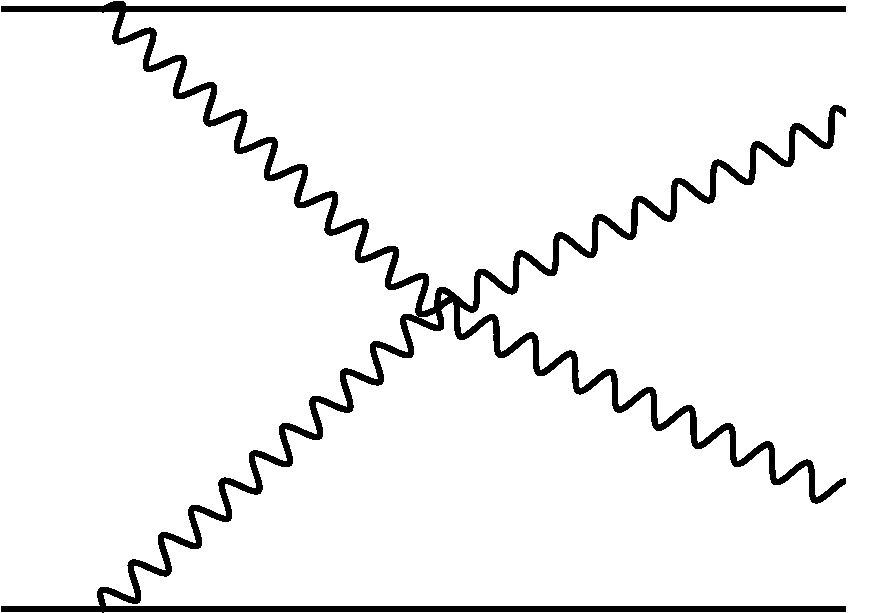
\includegraphics[width=0.3\textwidth,keepaspectratio]{figures/samples/feynVBS2.pdf}
}
\subfigure{
 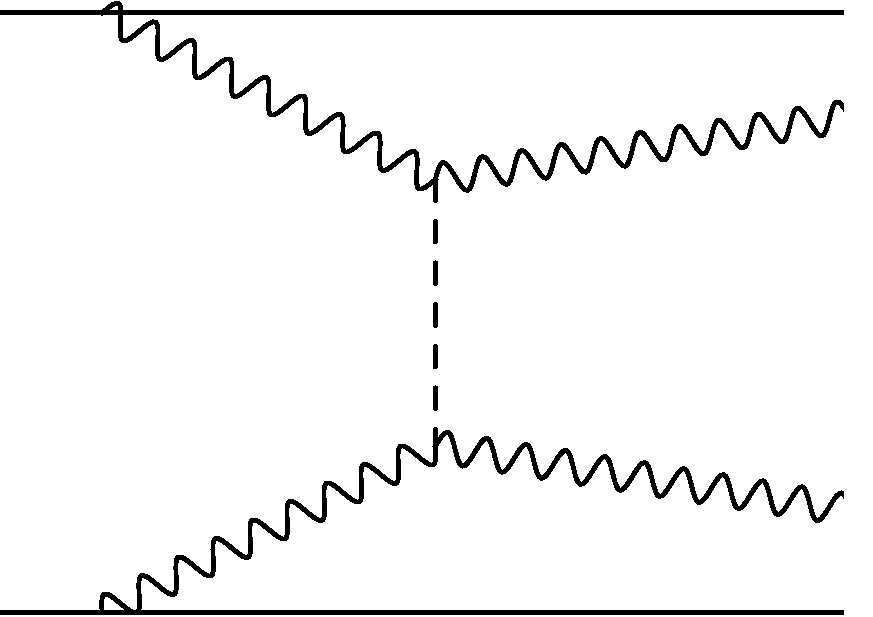
\includegraphics[width=0.3\textwidth,keepaspectratio]{figures/samples/feynVBS1.pdf}
}
\subfigure{
 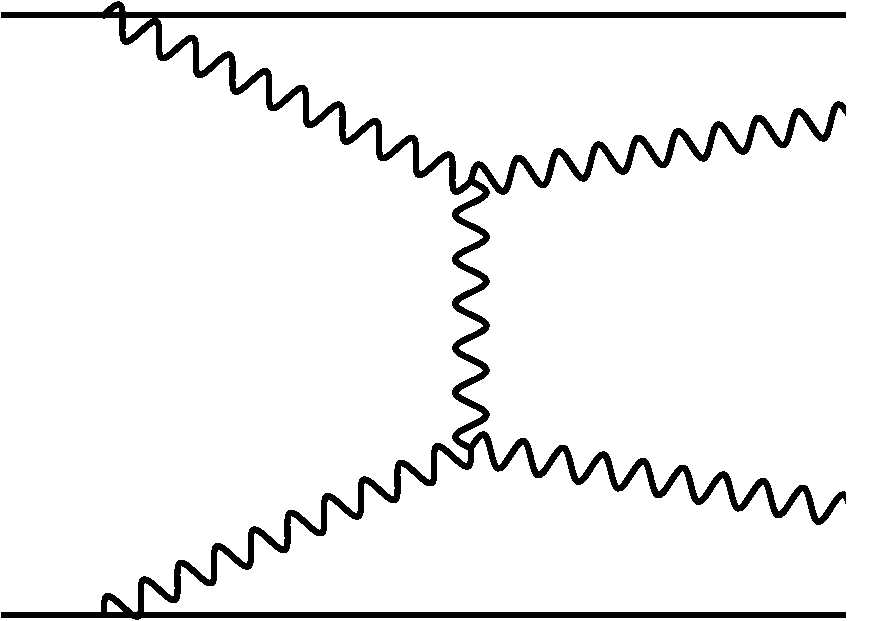
\includegraphics[width=0.3\textwidth,keepaspectratio]{figures/samples/feynVBS3.pdf}
}
\subfigure{
 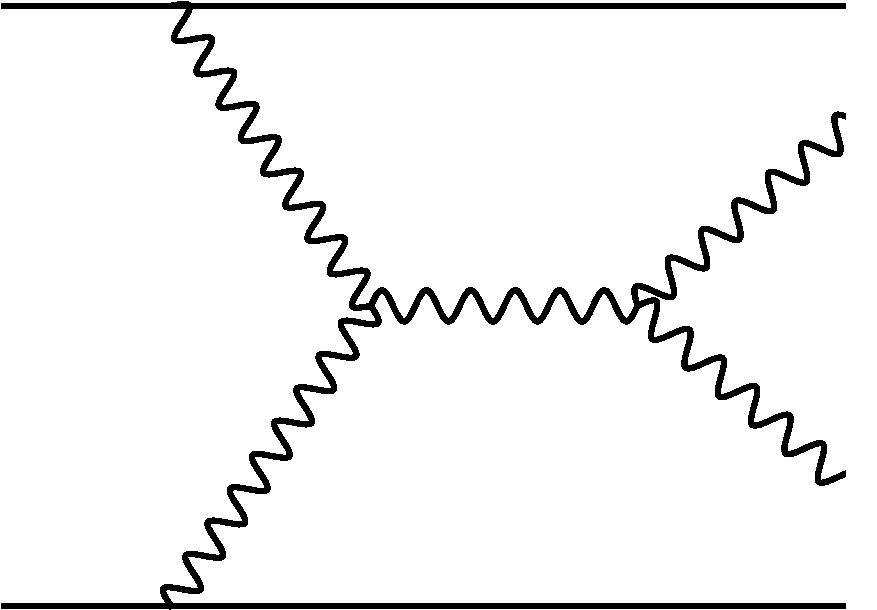
\includegraphics[width=0.3\textwidth,keepaspectratio]{figures/samples/feynVBS4.pdf}
}
\subfigure{
 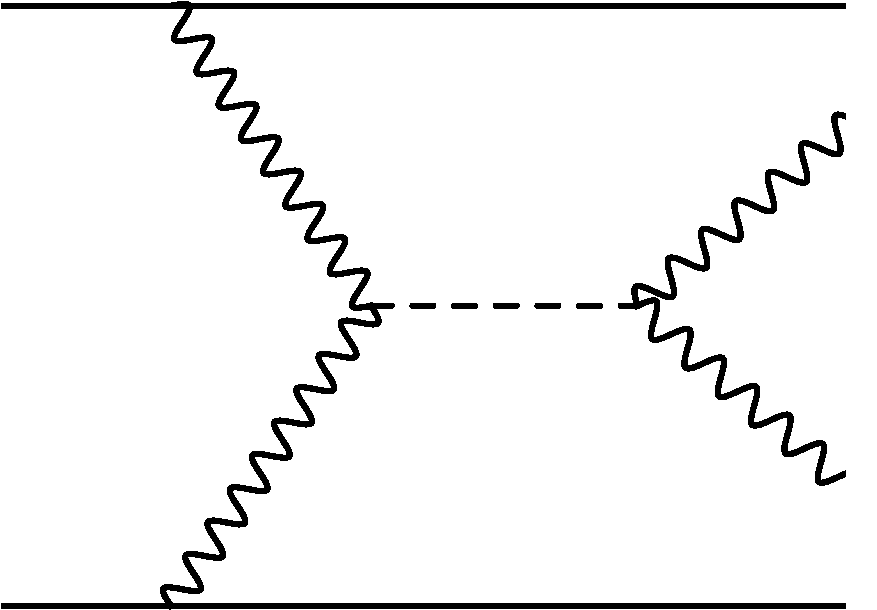
\includegraphics[width=0.3\textwidth,keepaspectratio]{figures/samples/feynVBS5.pdf}
}
\caption{
Examples of VBS diagrams that contribute to the signal.  Note that not all VBS diagrams contain quartic gauge couplings.
The dashed line represents the Higgs boson.  These and other Feynman diagrams in this note are made
using the JaxoDraw~\cite{Binosi:2003yf} program. The decays of the bosons are not shown.
}
\label{fig:feynmanVBS}
\end{center}
\end{figure}

%% feynman diagrams, non-VBS
%
\begin{figure}[tbp]
\begin{center}
\subfigure[]{
 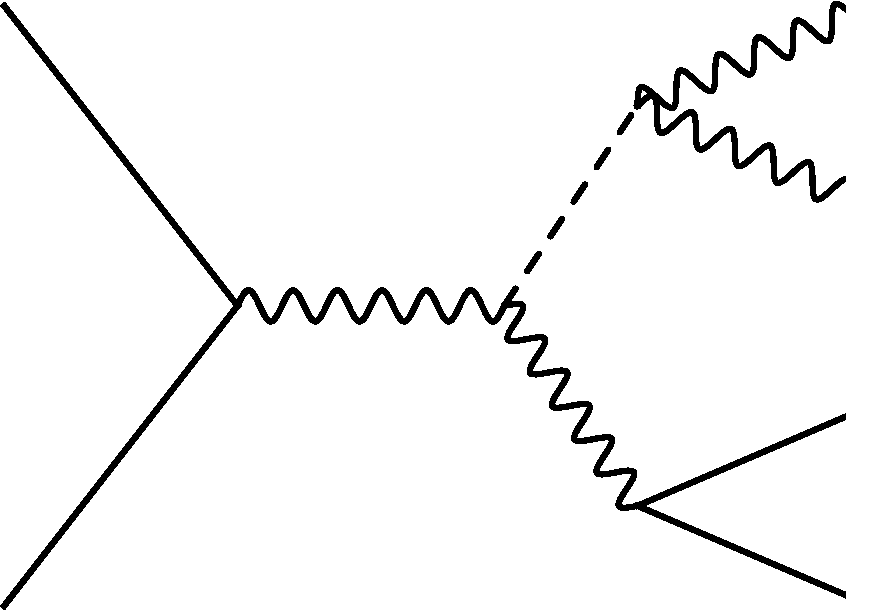
\includegraphics[width=0.3\textwidth,keepaspectratio]{figures/samples/feynEWKnonVBS3.pdf}
}
\subfigure[\label{subfig:feynEWKnonVBSb}]{
 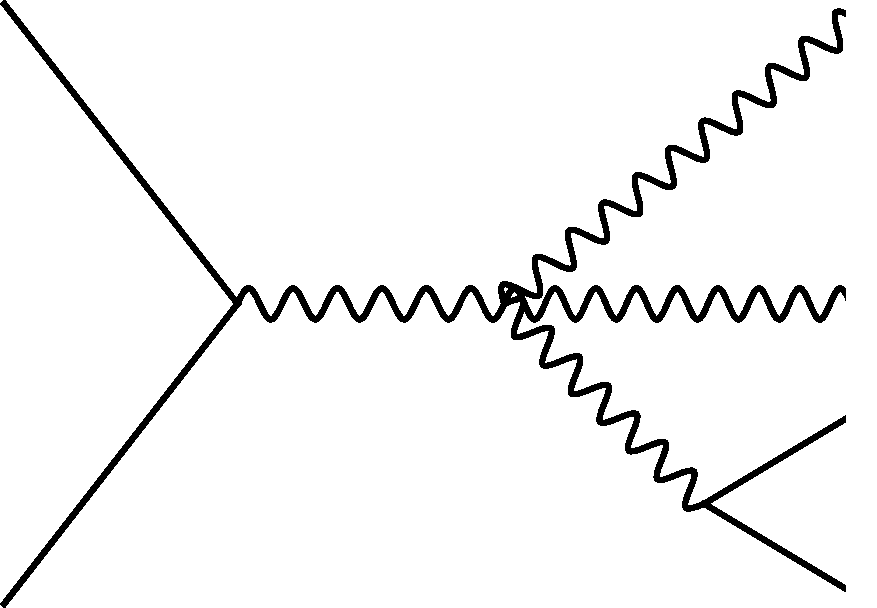
\includegraphics[width=0.3\textwidth,keepaspectratio]{figures/samples/feynEWKnonVBS4.pdf}
}
\subfigure[]{
 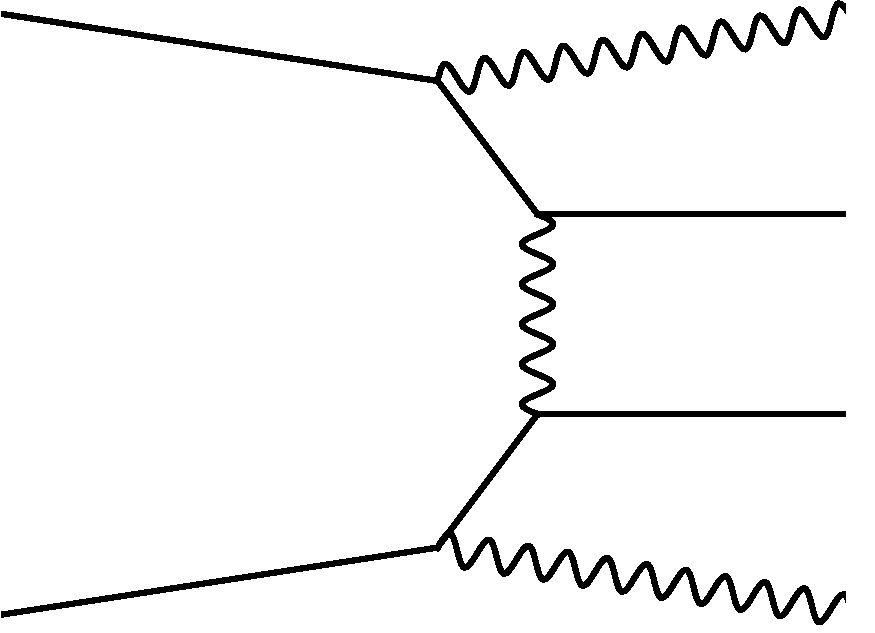
\includegraphics[width=0.3\textwidth,keepaspectratio]{figures/samples/feynEWKnonVBS5.pdf}
}
\subfigure[]{
 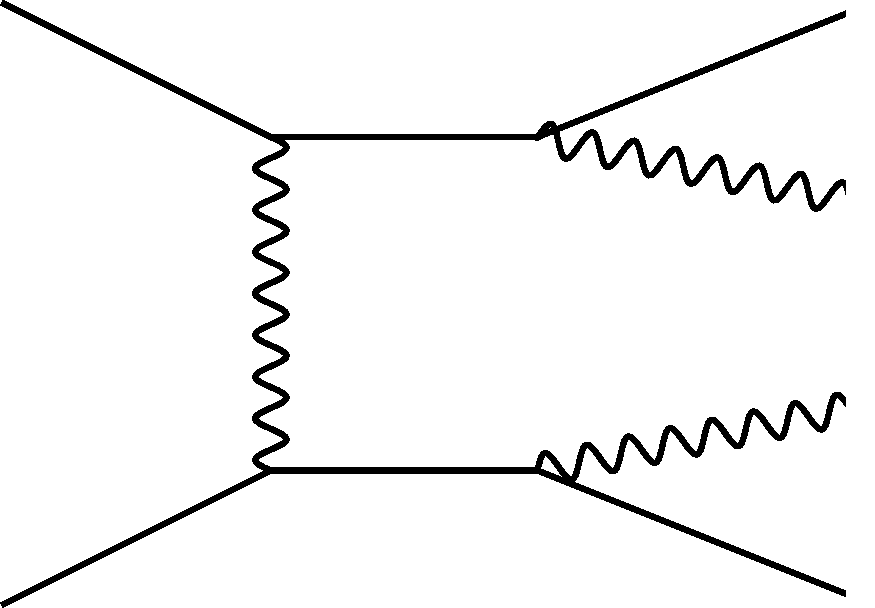
\includegraphics[width=0.3\textwidth,keepaspectratio]{figures/samples/feynEWKnonVBS6.pdf}
}
\subfigure[]{
 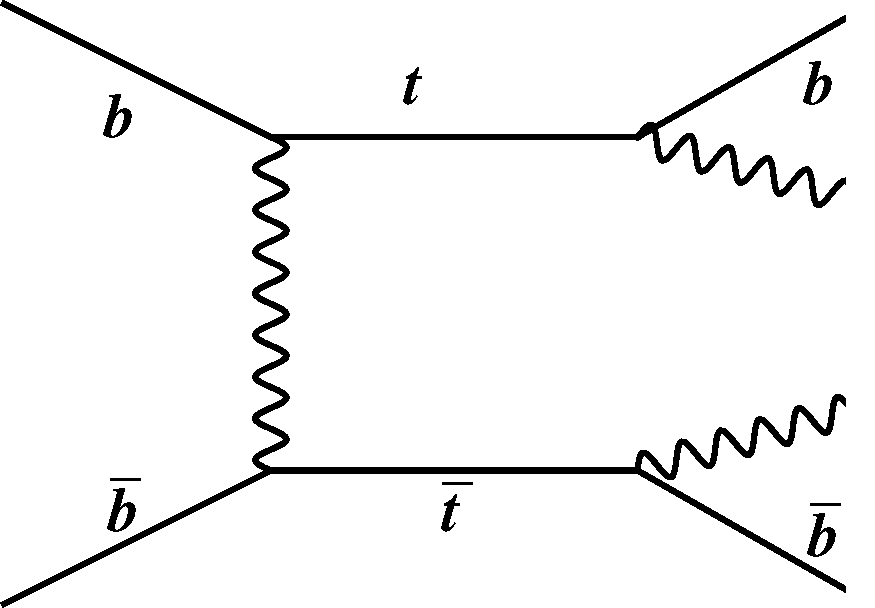
\includegraphics[width=0.3\textwidth,keepaspectratio]{figures/samples/feynEWKnonVBS1.pdf}
}
\subfigure[]{
 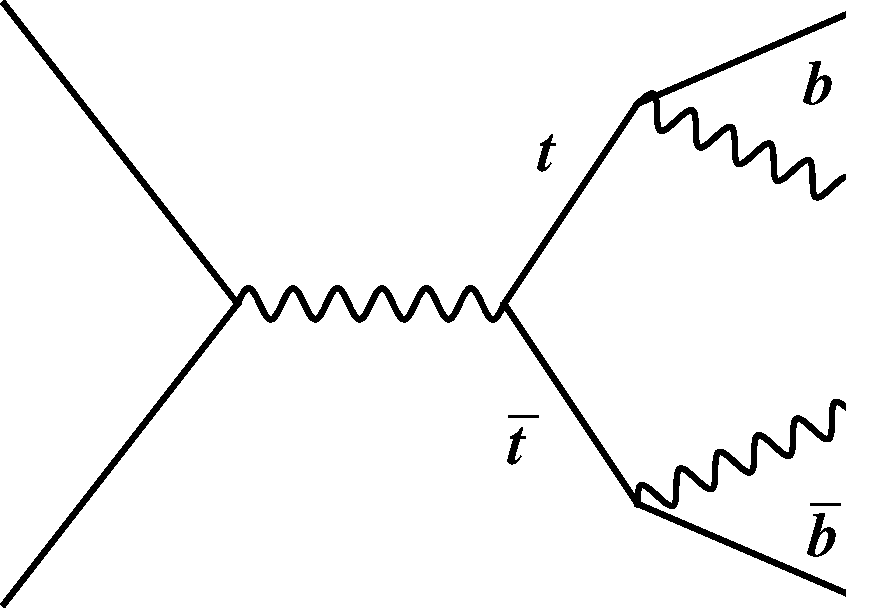
\includegraphics[width=0.3\textwidth,keepaspectratio]{figures/samples/feynEWKnonVBS2.pdf}
}
\subfigure[]{
 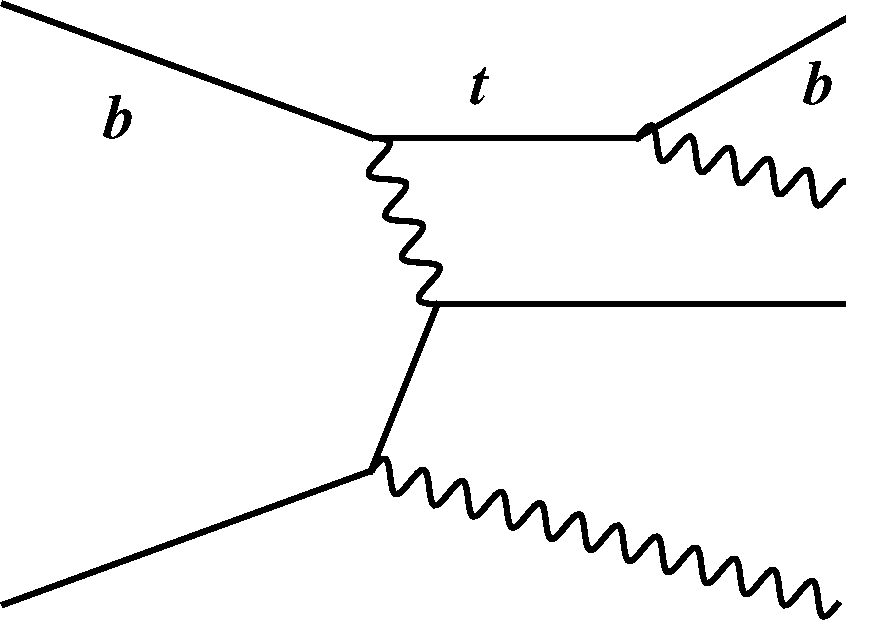
\includegraphics[width=0.3\textwidth,keepaspectratio]{figures/samples/feynEWKnonVBS7.pdf}
}
\caption{
Examples of non-VBS $\mathcal{O}(\alpha_{EW}^6)$ diagrams that contribute to the signal. The decays of the bosons are not
explicitly shown, but the counting of powers of $\alpha$ includes the boson decays.
}
\label{fig:feynmanEWKnonVBS}
\end{center}
\end{figure}

%% feynman diagram, tZb
\begin{figure}[tbp]
\begin{center}
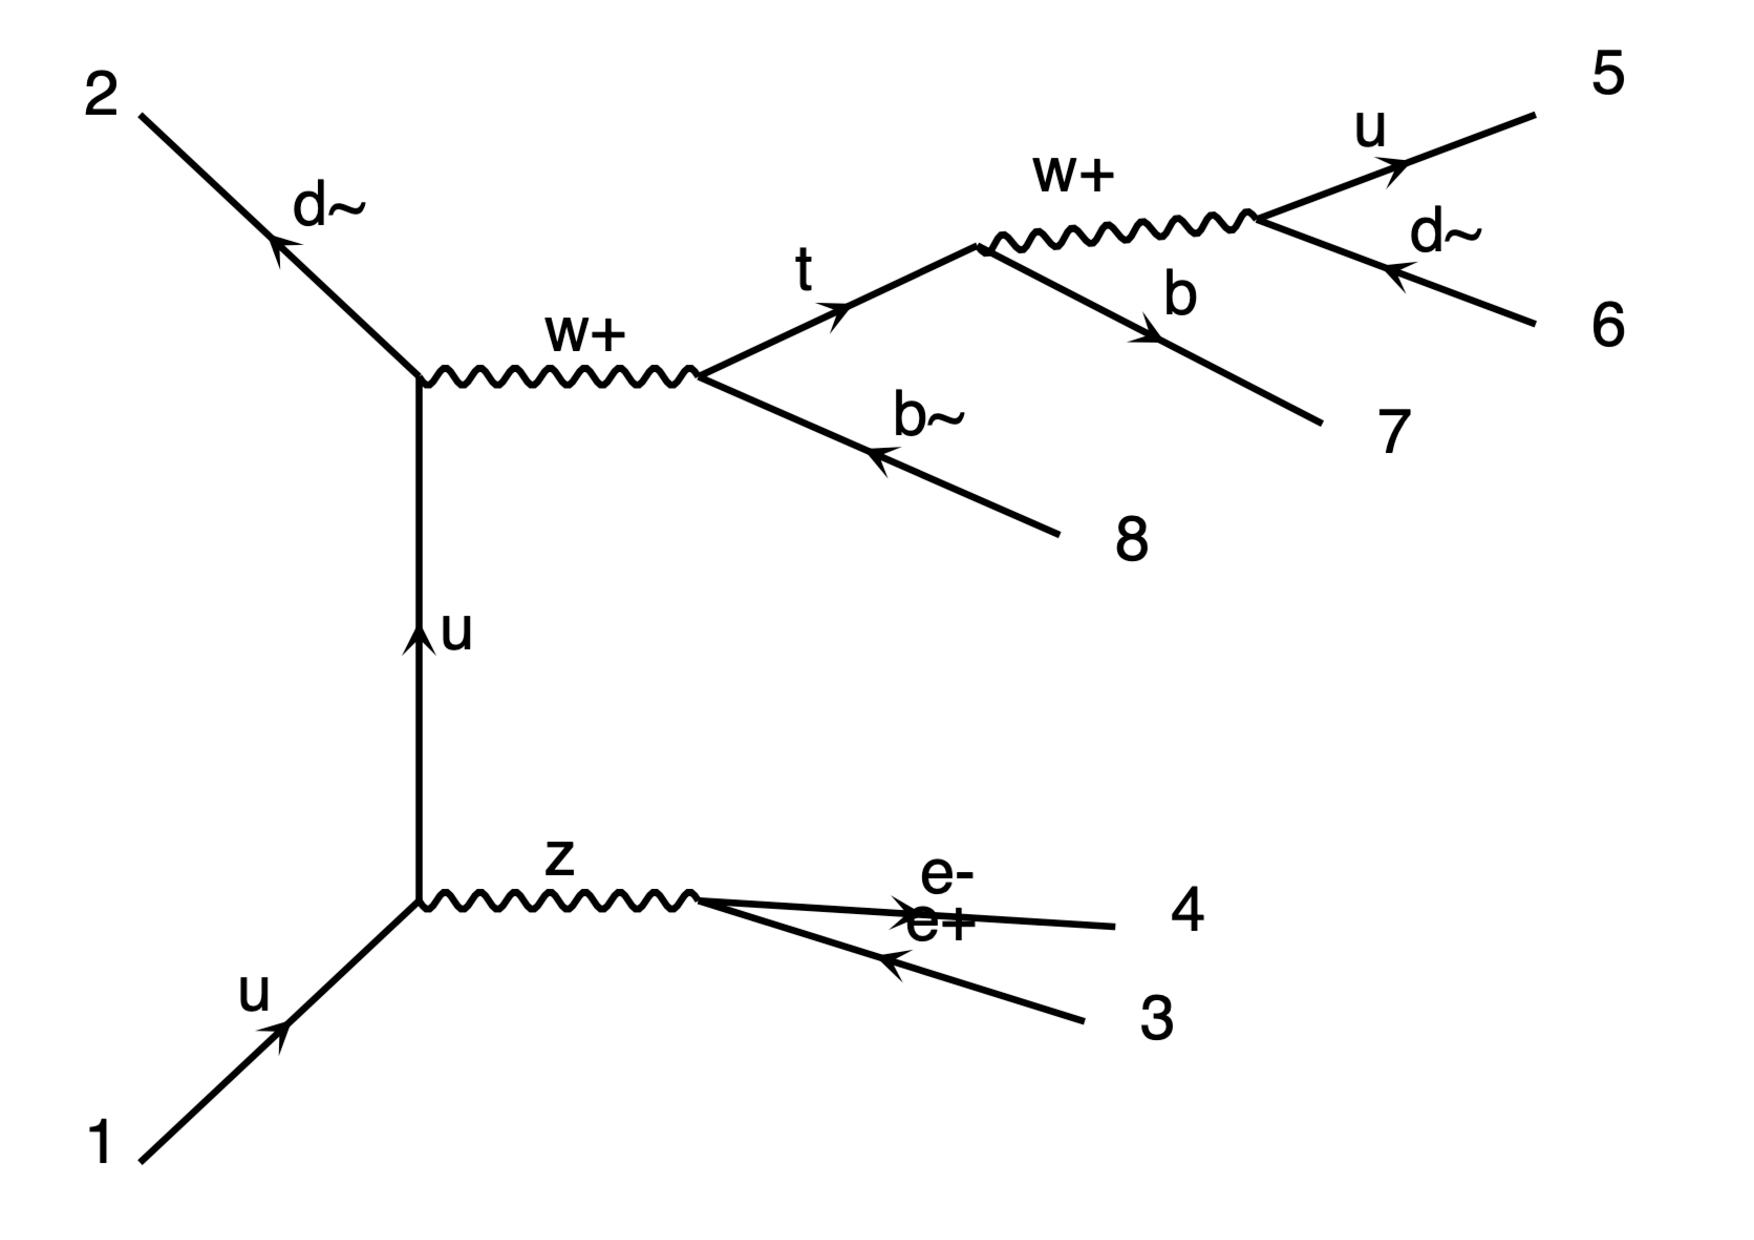
\includegraphics[width=0.3\textwidth,keepaspectratio]{figures/samples/feynEWKnonVBStZb.pdf}
\caption{
The example of the tZb diagram, which included in non-VBS $\mathcal{O}(\alpha_{EW}^6)$ diagrams.
}
\label{fig:feynmantZb}
\end{center}
\end{figure}

%% feynman diagrams, QCD
%
\begin{figure}[tbp]
\begin{center}
\subfigure[]{
 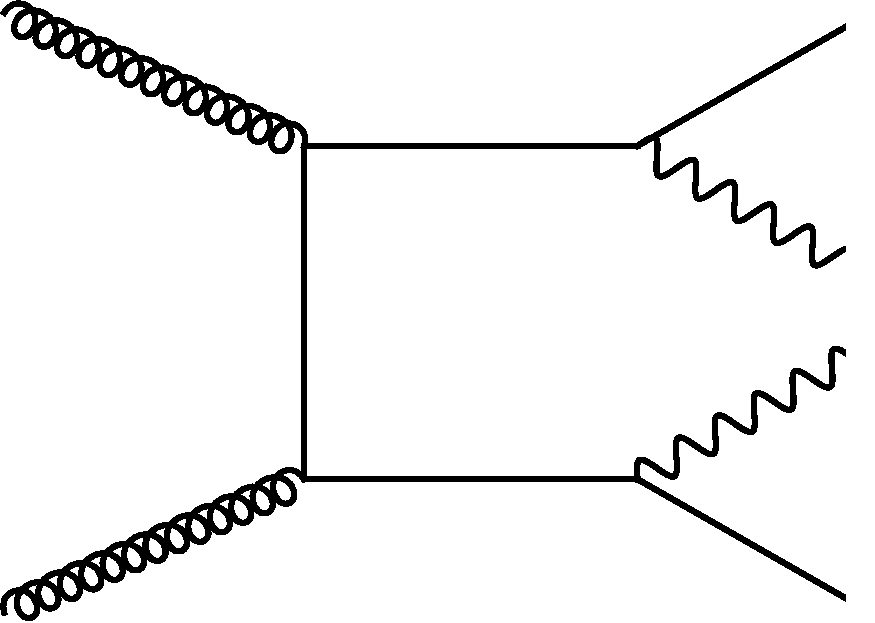
\includegraphics[width=0.3\textwidth,keepaspectratio]{figures/samples/feynQCD3.pdf}
}
\subfigure[]{
 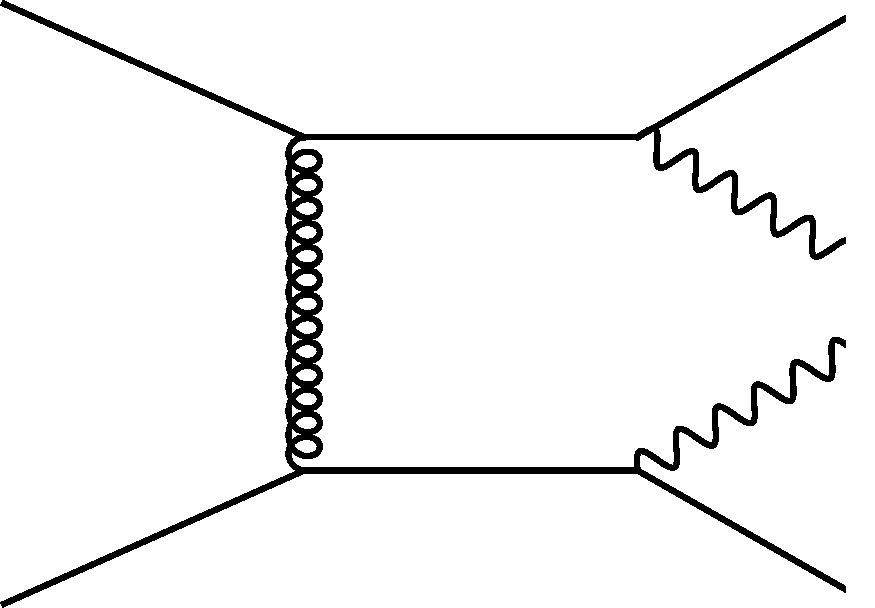
\includegraphics[width=0.3\textwidth,keepaspectratio]{figures/samples/feynQCD4.pdf}
}
\subfigure[]{
 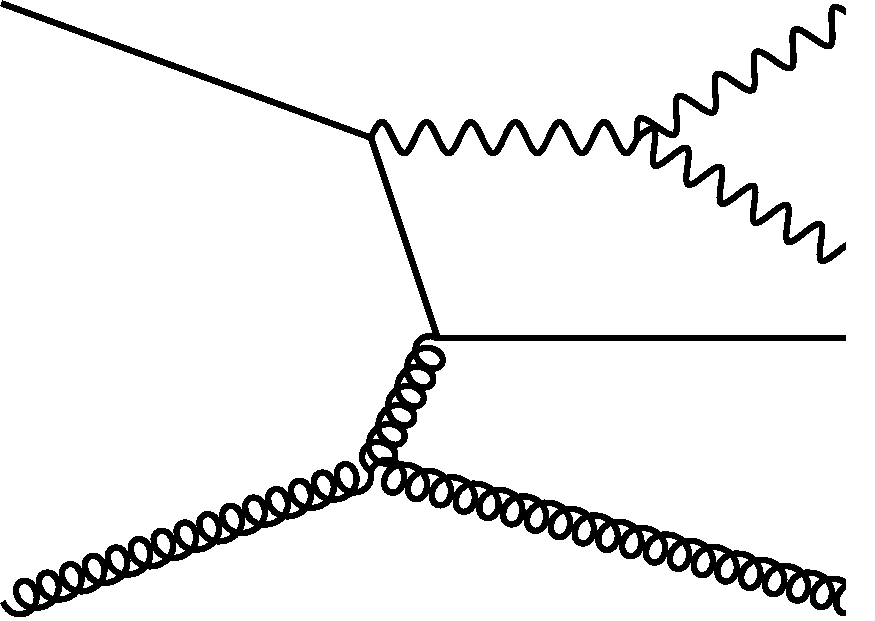
\includegraphics[width=0.3\textwidth,keepaspectratio]{figures/samples/feynQCD5.pdf}
}
\subfigure[]{
 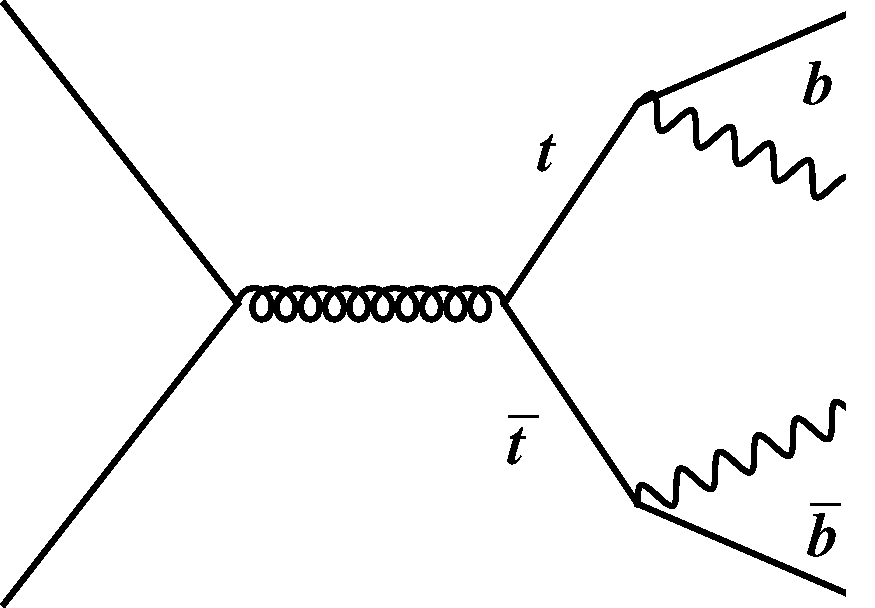
\includegraphics[width=0.3\textwidth,keepaspectratio]{figures/samples/feynQCD1.pdf}
}
\subfigure[]{
 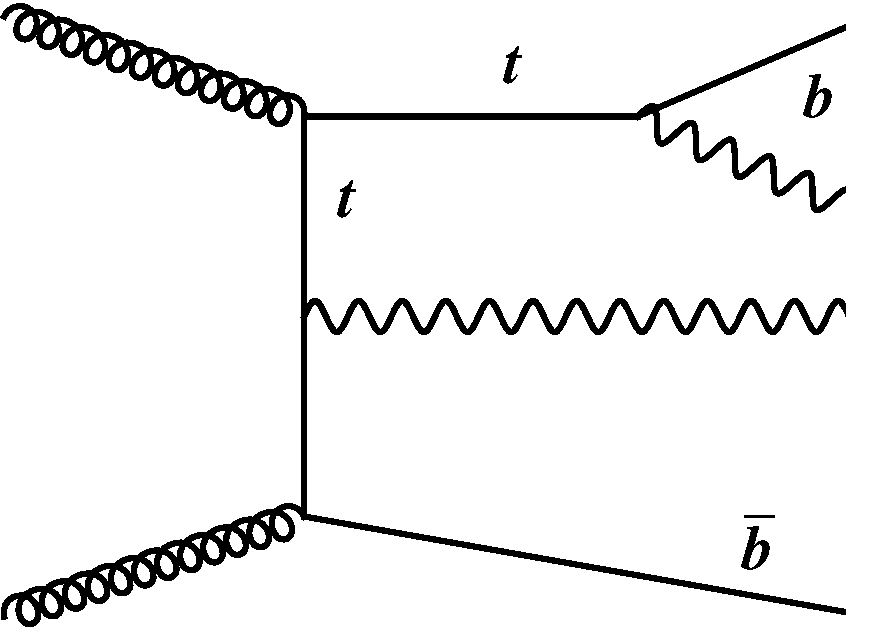
\includegraphics[width=0.3\textwidth,keepaspectratio]{figures/samples/feynQCD2.pdf}
}
\caption{
Examples of $\mathcal{O}(\alpha_{EW}^4 \alpha_{S}^2)$ diagrams that lead to the $VV$+2parton final state. These
are not included in the signal definition.  The decays of the bosons are not
explicitly shown, but the counting of powers of $\alpha$ includes the boson decays.
}
\label{fig:feynmanQCD}
\end{center}
\end{figure}
